% --------------------------------------------------------------------------------

\begin{exercise}[272]

Betrachten Sie die folgenden Eigenschaften, die eine Menge $A$ haben kann:

\begin{enumerate}[label = \alph*.]
  \item Es gibt eine injektive Abbildung von $\omega$ nach $A$. (\Quote{$\omega \leq A$})
  \item Es gibt eine fast injektive Abbildung von $\omega$ nach $A$.
  (\Quote{fast injektiv} bedeutet, dass das Urbild jedes Bildpunktes endlich ist.)
  \item Es gibt eine injektive, aber nicht surjektive Abbildung von $A$ nach $A$.
  \item Es gibt eine fast injektive, aber nicht surjektive Abbildung von $A$ nach $A$.
  \item Für ein (alle) $x \notin A$ gibt es eine Bijektion von $A$ nach $A \cup \Bbraces{x}$.
  (\Quote{$A = A + 1$})
  \item Es gibt eine surjektive, aber nicht injektive Abbildung von $A$ nach $A$.
  \item Es gibt eine surjektive Abbildung von $A$ auf $\omega$. (\Quote{$\omega \leq^* A$})
  \item Es gibt eine surjektive, fast injektive Abbildung von $A$ auf $\omega$.
  \item Es gibt eine injektive Abbildung von $\omega$ nach $P(A)$. (\Quote{$\omega \leq P(A)$})
  \item Es gibt eine injektive Abbildung von $\omega$ in die endlichen Teilmengen von $A$. (\Quote{$\omega \leq P_\mathrm{fin}(A)$})
  \item Es gibt eine surjektive Abbildung von den endlichen Teilmengen von $A$ auf $\omega$.
  \item $A$ ist unendlich: \Quote{$|A| = \infty$}
  \item Es gibt eine nichtleere Teilmenge von $\mathfrak{P}(A)$ ohne (bez. $\subseteq$) maximales Element.
\end{enumerate}

Geben Sie möglichst viele nichttriviale Implikationen zwischen diesen Aussagen an, die sich in ZF (also ohne Auswahlaxiom) beweisen lassen.

\end{exercise}

% --------------------------------------------------------------------------------

\begin{solution}

\phantom{}

\begin{enumerate}[label = \texttt{ad}]

  \item \Quote{a. $\implies$ b.}:

  Klar!

  \item \Quote{b. $\implies$ a.}:
  
  \begin{enumerate}[label = \arabic*.]

    \item Lösung:
    
    Sei $f: \omega \to A$ fast injektiv, d.h.

    \begin{align*}
      \Forall x \in f[\omega]:
      |f^{-1}[\Bbraces{x}]| < \infty.
    \end{align*}

    Wir fassen $\omega$ und $A$ als Algebren mit leerem Typ auf.
    Auf diese können wir also den Homomorphiesatz anwenden und bekommen eine Abbildung $g$.

    \textbf{Achtung!}
    Möglicherweise braucht der Homomorphiesatz das Auswahlaxiom?
    Anstatt einen beliebigen Repräsentanten $u$ von $U$ zu wählen, kann man in unserem Fall den kleinsten $u := \min U$ (von endlich vielen) wählen, um $g(U) := f(u)$ zu definieren.
    Wir haben es schließlich mit Schuhen und nicht mit Socken zu tun!

    \phantom{}

    \begin{tcolorbox}[standard jigsaw, opacityback = 0]
      \centering
      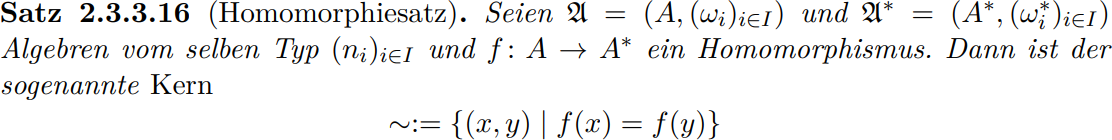
\includegraphics
      [width = 0.75 \textwidth]
      {Alg/Alg - Satz 2.3.3.16.1 (Homomorphiesatz).png} \\
      \vspace{0.25 cm}
      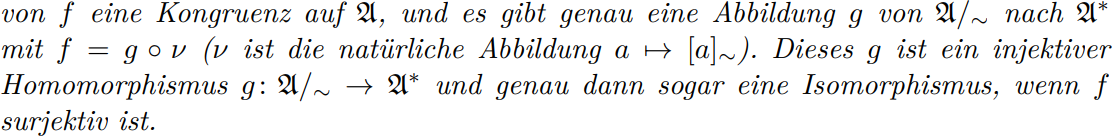
\includegraphics
      [width = 0.75 \textwidth]
      {Alg/Alg - Satz 2.3.3.16.2 (Homomorphiesatz).png} \\
      \vspace{0.25 cm}
      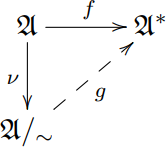
\includegraphics
      [width = 0.15 \textwidth]
      {Alg/Alg - Satz 2.3.3.16.3 (Homomorphiesatz).png}
    \end{tcolorbox}

    \phantom{}

    Seien die (unendlich vielen!) Urbilder gemäß ihrem Minimum, vermöge $h$ (strikt monoton steigend), geordnet, d.h.

    \begin{align*}
      h := (U_n)_{n \in \omega}:
      \omega \to \omega / \sim:
      \min U_1 < \min U_2 < \cdots
    \end{align*}

    $g \circ h: \omega \to A$ ist, als Verkettung injektiver Funktionen, injektiv.

    \item Lösung:

    Sei $f: \omega \to A$ fast injektiv. \\
    Definiere die injektive Funktion $f': \omega \to A$ durch
    \begin{align*}
      f'(0) &:= f(0) \\
      f'(n) &:= f(\min\{k \in  \N:  f(k) \notin f[\{0,\dots,k-1\}]\}), \quad n \geq 1.
    \end{align*}
    Da das Urbild jedes Bildpunktes endlich ist, exisitiert dieses Minimum immer.

  \end{enumerate}

  \item \Quote{a. $\implies$ c.}: Sei $f: \omega \to A$ injektiv.
  Definiere
  \begin{align*}
    g := \{(f(n),f(n+1)): n \in \omega\} \cup \{(a,a): a \in A \setminus f(\omega)\}
  \end{align*}
  $g$ ist sicher auf ganz $A$ definiert, injektiv und es gilt $f(0) \notin g(A)$.

  \item \Quote{a. $\implies$ f.}: Sei $f: \omega \to A$ injektiv. Definiere

  \begin{align*}
    g := \{(f(n+1),f(n)): n \in \omega\} \cup \{(a,a): a \in A \setminus f(\omega)\}
    \cup \{(f(0),f(0))\}
  \end{align*}
  $g$ ist surjektiv, aber nicht injektiv.

  \item \Quote{c. $\implies$ a.}: Siehe letzte Übung.

  \item \Quote{a. $\implies$ h.}: Sei $f: \omega \to A$ injektiv. Definiere
  \begin{align*}
    g = \{(f(n), n): n \in \omega\} \cup \{(a,0): a \in A \setminus f(\omega)\}.
  \end{align*}

  \item \Quote{c. $\implies$ d.}:

  Klar.

  \item \Quote{e. $\implies$ c.}:

  Sei $x \not \in A$ und $f: A \to A \cup \Bbraces{x}$ bijektiv.
  $f^{-1} |_A: A \to A$ ist injektiv, trifft aber nicht $f^{-1}(x)$, ist also nicht surjektiv.

  \item \Quote{e. $\implies$ f.}:

  Sei $x \not \in A$ und $f: A \to A \cup \Bbraces{x}$ bijektiv.
  Sei weiters $y \in A$.
  $g: A \to A$ ist surjektiv, $y$ hat aber die beiden verschiedenen Urbilder $f^{-1}(y) \neq f^{-1}(x)$, weil $x \neq y$, ist also nicht injektiv.

  \begin{align*}
    g:
    A \to A:
    z
    \mapsto
    \begin{cases}
      f(z), & f(z) \in A, \\
      y,    & f(z) = x
    \end{cases}
  \end{align*}

  \item \Quote{a. $\implies$ g.}:
  
  Sei $f: \omega \to A$ injektiv.
  Es gibt folglich also eine (surjektive) Linksinverse $f^{-1}: f[\omega] \to \omega$.
  Wir setzen diese zu einer (surjektiven) Funktion $g: A \to \omega$ beliebig fort.

  \item \Quote{h. $\implies$ g.}:
  
  Klar!

  \item \Quote{a. $\implies$ j.}:

  Sei $f: \omega \to A$ injektiv, so auch $g: \omega \to P_\mathrm{fin}(A): n \to \Bbraces{n}$.

  \item \Quote{j. $\implies$ i.}:

  Klar!

  \item \Quote{j. $\implies$ k.}:

  Verwende \Quote{a. $\implies$ g.} für $P_\mathrm{fin}(A)$ anstelle von $A$.

  \item \Quote{g. $\implies$ k.}:

  Sei $f: A \to \omega$ surjektiv.

  \begin{gather*}
    g:
    P(A) \to \omega:
    M \mapsto \min f[M],
    \quad
    g_\mathrm{fin} := g |_{P_\mathrm{fin}(A)},
    \quad
    g_\mathrm{sing} := g_\mathrm{fin} |_{P_\mathrm{sing}(A)} \cong f \\
    \implies
    \omega
    \supseteq
    g(P(A))
    \supseteq
    g_\mathrm{fin}(P_\mathrm{fin}(A))
    \supseteq
    g_\mathrm{sing}(P_\mathrm{sing}(A))
    =
    f(A)
    =
    \omega
  \end{gather*}

  $g$, $g_\mathrm{fin}$, und $g_\mathrm{sing}$ sind also auch allersamt surjektiv.

\end{enumerate}

\end{solution}

% --------------------------------------------------------------------------------
